\documentclass[a4paper,english,11pt,twoside]{article}
\usepackage[utf8]{inputenc}
\usepackage[T1]{fontenc}
\usepackage[english]{babel}
\usepackage{epsfig}
\usepackage{graphicx}
\usepackage{amsmath}
\usepackage{pstricks}
\usepackage{subfigure}
\usepackage{booktabs}
\usepackage{float}
\usepackage{gensymb}
\usepackage{preamble}
\restylefloat{table}
\renewcommand{\arraystretch}{1.5}
 \newcommand{\tab}{\hspace*{2em}}


\date{\today}
\title{Mandatory Assignment 2}
\author{Jørgen D. Tyvand}

\begin{document}
\maketitle
\newpage

\section*{i)}
Equation (170) states:\\
\\
(170)$\tab f''' + ff'' + \beta(1 - (f')^2) = 0$\\
\\
where $\beta$ is a constant.\\
\\
This is solved similarly to the plane stagnation flows from Mandatory 1, as this is the same equation with the added constant $\beta$ in front of the last term.\\
\\
We start again by defining $h = f'$, and get a system of coupled equations:\\
\\
$h - f' = 0$\\
$h'' + fh' + \beta(1 - h^2) = 0$\\
\\
Since the two equations only wary by a constant in the last term, the variational form becomes the same as for equation (146), just with the added constant for the two terms from the parenthesis:\\
\\
$\int\limits_{\Omega}hv_fdx +\int\limits_{\Omega}\nabla f v_fdx - \int\limits_{\Omega}\nabla h\cdot\nabla v_hdx + \\
\\
\int\limits_{\Omega} f \nabla h v_hdx + \beta\int\limits_{\Omega}v_hdx - \beta\int\limits_{\Omega}h^2v_hdx = 0$\\
\\
\\
The solver is implemented as follows:
\\
\begin{lstlisting}[style=python]
from dolfin import *
from numpy import zeros,diff
import matplotlib.pyplot as plt
set_log_active(False)

L = 6.
Beta = [1.,0.3,0,-0.1,-0.18,-0.198838]
mesh = IntervalMesh(10000, 0, L)
V = FunctionSpace(mesh, 'CG', 1)
VV = V * V
vf, vh = TestFunctions(VV)

bc0 = DirichletBC(VV, Constant((0,0)), 
	"std::abs(x[0]) < 1e-12")
bc1 = DirichletBC(VV.sub(1), Constant(1), 
	"std::abs(x[0]-%d) < 1e-12" % L)

xfunc = Function(V)
xfunc = interpolate(Expression("x[0]"),V)
xvals = xfunc.compute_vertex_values()
xdiff = xvals[1]-xvals[0]
hdx = []

plt.figure()
for beta in Beta:
	fh_=interpolate(Expression(("x[0]","1./L*x[0]"),
				L=L),VV)
	f_,h_=split(fh_)
	F = h_*vf*dx - f_.dx(0)*vf*dx - inner(grad(h_), 
		grad(vh))*dx + f_*h_.dx(0)*vh*dx + 
		beta*vh*dx - beta*h_**2*vh*dx
	solve(F==0, fh_ , [bc0, bc1])

	f_,h_= fh_.split(True)
	
	hvals = h_.compute_vertex_values()
	
	hdiff = project(h_.dx(0),V)
	hdx.append(hdiff.compute_vertex_values())

	plt.plot(xvals, hvals, label='$ \\beta=%f $' % beta)
	plt.legend(loc='center right')

plt.xlabel(r'$ \eta = y \sqrt{U(1+m)/2 \nu x} $')
plt.ylabel("f'")
plt.axis([0, 6, 0, 1.2])

plt.figure()
for i in range(len(hdx)):
	plt.plot(xvals,hdx[i], label='$ \\beta=%f $' % Beta[i])
	plt.legend(loc='center right')

plt.xlabel(r'$ \eta = y \sqrt{U(1+m)/2 \nu x} $')
plt.ylabel("f''")
plt.axis([0, 6, 0, 1.4])
plt.show()
\end{lstlisting}

\newpage
\section*{a)}
The solver gives the two following plots, cloesly resembling Fig. 4-11 (a) and (b) in White:\\
\begin{figure}[h!]
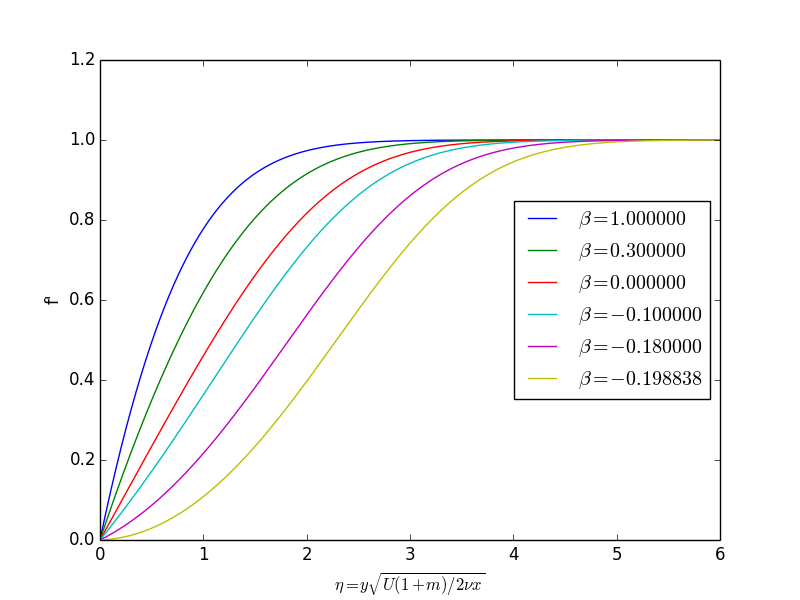
\includegraphics[scale=0.6]{1a_figure_1.png}
\end{figure}
\begin{figure}[h!]
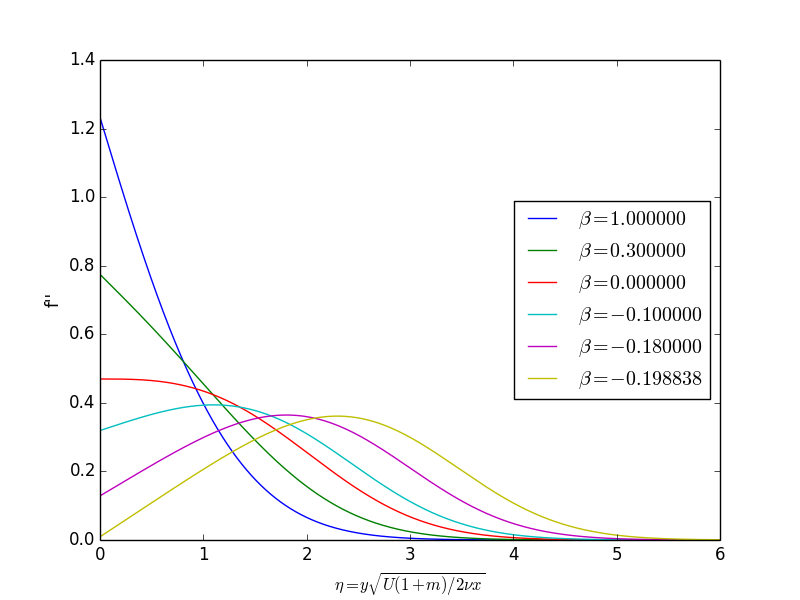
\includegraphics[scale=0.6]{1a_figure_2.png}
\end{figure}
\\
\section*{b)}
Using the solver from a), and testing for $\beta=-0.19884$, we get the following plot:
\\
\begin{figure}[h!]
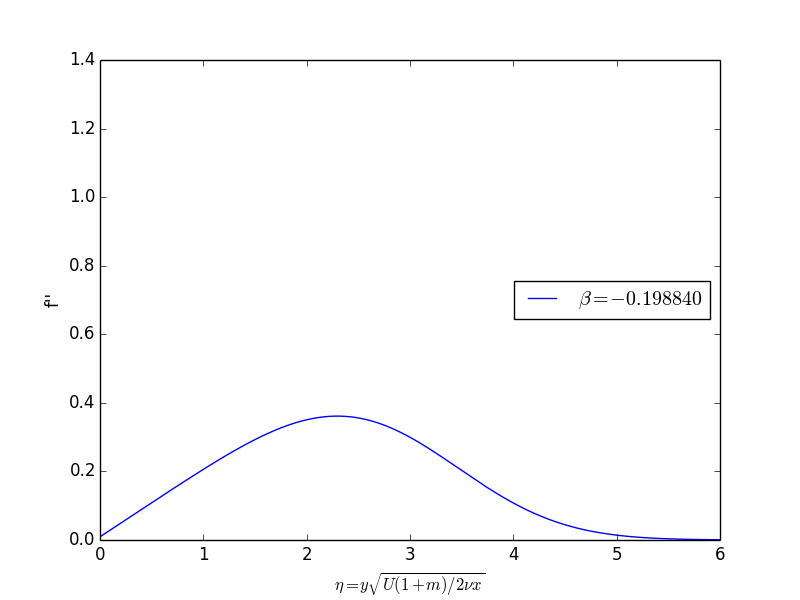
\includegraphics[scale=0.7]{1b_figure_1.png}
\end{figure}
\\
White states that $f''$ should be zero for  $\beta=-0.19884$, while the computed value is 0.00935 using 10000 mesh nodes. Therefore we can, while still using 10000 nodes, go slightly below -0.19884 and still get a result for $f''$:\\
\begin{lstlisting} [style=terminal]
beta = -0.198900, f'' = 0.006891
beta = -0.198950, f'' = 0.003990
beta = -0.198970, f'' = 0.002157
beta = -0.198975, f'' = 0.001493
beta = -0.198979, f'' = 0.000788
\end{lstlisting}
While it fails to find a solution for $\beta = -0.19898$. Increasing the mesh size does not yeild a much better result, and fails to converge at around  24900+ mesh points. (still with $f''$ at around 0.0093).\\
\\
Running the solver twice for $\beta=-0.1$, and using the initial guess with a negative sign as the guess for the negative solution, we get the following plot for the two solutions:\\
\begin{figure}[h!]
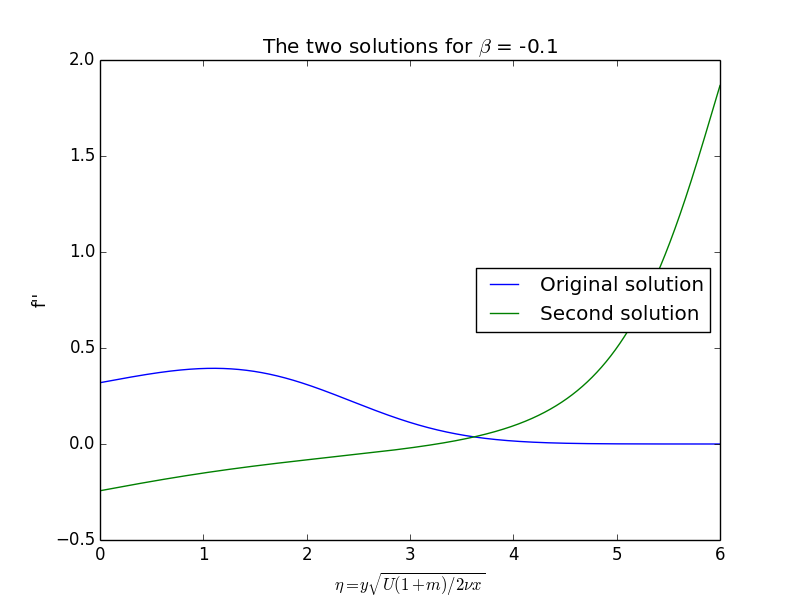
\includegraphics[scale=0.7]{1b_figure_2.png}
\end{figure}

\section*{ii a)}
The solver for the steady case is given below:\\
\begin{lstlisting}[style=python]
from dolfin import *
from numpy import eye
set_log_active(False)

H = 0.41
D = 0.1
R = D/2.
Um = 0.3
nu = 0.001
rho = 1

mesh = Mesh('prob2.xml')
i = 4
for i in range(i):
	mesh = refine(mesh)

	n = -FacetNormal(mesh)
	n1 = as_vector((1.0,0))
	n2 = as_vector((0,1.0))
	nx = dot(n,n1)
	ny = dot(n,n2)
	nt = as_vector((ny,-nx))

	V = VectorFunctionSpace(mesh, 'CG', 2)
	Q = FunctionSpace(mesh, 'CG', 1)
	VQ = V * Q
	ug, pg = TrialFunctions(VQ)
	vg, qg = TestFunctions(VQ)
	u, p = TrialFunctions(VQ)
	v, q = TestFunctions(VQ)

	def top(x, on_boundary): return x[1] > (H-DOLFIN_EPS)
	def bottom(x, on_boundary): return x[1] < DOLFIN_EPS
	def circle(x, on_boundary): return sqrt((x[0]-0.2)**2 
					+ (x[1]-0.2)**2) < 
					(R+DOLFIN_EPS)

	u_in = Expression(("4*Um*x[1]*(H-x[1])/(H*H)","0.0"),
					Um=Um,H=H)

	bc0 = DirichletBC(VQ.sub(0), Constant((0,0)), top)
	bc1 = DirichletBC(VQ.sub(0), Constant((0,0)), bottom)
	bc2 = DirichletBC(VQ.sub(0), Constant((0,0)), circle)
	inflow  = DirichletBC(VQ.sub(0), u_in, 
					"x[0] < DOLFIN_EPS")
	bcs = [bc0, bc1, bc2, inflow]

	Fg = rho*nu*inner(grad(vg), grad(ug))*dx - 
		div(vg)*pg*dx - q*div(ug)*dx + 
		Constant(0)*qg*dx

	upg_ = Function(VQ)
	solve(lhs(Fg)==rhs(Fg), upg_, bcs=bcs)

	up_1 = Function(VQ)
	k = 0
	error = 1
	while k < 10 and error > 1e-5:

		F = rho*nu*inner(grad(u), grad(v))*dx + 
			rho*inner(grad(u)*upg_.sub(0),v)*dx - 
			div(v)*p*dx - q*div(u)*dx + 
			Constant(0)*q*dx
		solve(lhs(F)==rhs(F), up_1, bcs=bcs)
		error = errornorm(upg_, up_1)
		upg_.assign(up_1)
		k += 1

	u_,p_ = upg_.split(True)


	Circle = AutoSubDomain(circle)
	mf = FacetFunction("size_t", mesh)
	mf.set_all(0)
	Circle.mark(mf, 1)
	ds = ds[mf]

	ut = dot(nt,u_)
	Uav = (2*Um)/3
	Fd = assemble((rho*nu*dot(grad(ut),n)*ny-p_*nx)*ds(1), 
		exterior_facet_domains=mf, mesh=mesh)
	Fl = assemble(-(rho*nu*dot(grad(ut),n)*nx+p_*ny)*ds(1), 
		exterior_facet_domains=mf, mesh=mesh)
	Cd = (2*Fd)/(rho*Uav**2*D)
	Cl = (2*Fl)/(rho*Uav**2*D)

	press = p_.compute_vertex_values()
	dp = press[5]-press[7]

	u,v = u_.split(True)
	uvals = u.compute_vertex_values()
	xmax = 0
	for j in range(len(uvals)):
		if uvals[j] < 0:
			if mesh.coordinates()[j][0] > xmax:
				xmax = mesh.coordinates()[j][0]
	La = xmax - 0.25
	print('Unknowns = %d, Cd = %f, Cl = %f, dp = %f 
		La = %f' % (len(mesh.coordinates()), 
		Cd, Cl, dp, La))
\end{lstlisting}

The program finds an initial guessed solution by solving the problem without the convection term. The convection term is then added in a new form, and solved using Picard iterations with the guess inserted into the convection term. The whole program runs four times, refining an initial mesh and giving the following values for $C_D$, $C_L$, $L_a$ and $\Delta P$:\\
\\
\begin{lstlisting} [style=terminal]
Unknowns: 1006  Cd: 5.5136 Cl: 0.0116, dp: 0.1170 La: 0.0749
Unknowns: 3852  Cd: 5.5405 Cl: 0.0115, dp: 0.1174 La: 0.0819
Unknowns: 15064 Cd: 5.5505 Cl: 0.0109, dp: 0.1175 La: 0.0819
Unknowns: 59568 Cd: 5.5551 Cl: 0.0106, dp: 0.1176 La: 0.0836
\end{lstlisting}
Comparing this to Table 3, we see that the computed results are reasonable values.

\newpage
\section*{ii b)}
For the unsteady case, I have used the code from the Navier-Stokes demo from Fenics Project as a base for the solver. The completed code is given below:\\
\begin{lstlisting}[style=python]
from dolfin import *
from numpy import zeros, savetxt, column_stack
import matplotlib.pyplot as plt
import sys
set_log_active(False)

# Print log messages only from the root process in parallel
parameters["std_out_all_processes"] = False;

# Load mesh from file
mesh = Mesh("prob2.xml")
i = 2
for i in range(i):
	mesh = refine(mesh)
print len(mesh.coordinates())

n = -FacetNormal(mesh)
n1 = as_vector((1.0,0))
n2 = as_vector((0,1.0))
nx = dot(n,n1)
ny = dot(n,n2)
nt = as_vector((ny,-nx))

# Define function spaces (P2-P1)
V = VectorFunctionSpace(mesh, "CG", 2)
Q = FunctionSpace(mesh, "CG", 1)

# Define trial and test functions
u = TrialFunction(V)
p = TrialFunction(Q)
v = TestFunction(V)
q = TestFunction(Q)

# Set parameter values
dt = 0.0005
T = 0.331
nu = 0.001
rho = 1
Um = 1.5
Uav = (2*Um)/3
H = 0.41
D = 0.1
R = D/2.
St = (D*(1/T))/Uav


# Define velocity boundary condition
u_in = Expression(("4*Um*x[1]*(H-x[1])/(H*H)","0.0"),Um=Um,H=H)

# Define boundary conditions
def top(x, on_boundary): return x[1] > (H-DOLFIN_EPS)
def bottom(x, on_boundary): return x[1] < DOLFIN_EPS
def circle(x, on_boundary): return sqrt((x[0]-0.2)**2 + 
			     (x[1]-0.2)**2) < (R+DOLFIN_EPS)

bc0 = DirichletBC(V, Constant((0,0)), top)
bc1 = DirichletBC(V, Constant((0,0)), bottom)
bc2 = DirichletBC(V, Constant((0,0)), circle)

inflow  = DirichletBC(V, u_in, "x[0] < DOLFIN_EPS")
outflow = DirichletBC(Q, 0, "x[0] > 2.2 - DOLFIN_EPS")
bcu = [bc0, bc1, bc2, inflow]
bcp = [outflow]

# Create functions
u0 = Function(V, 'u0.xml')
u1 = Function(V)
p1 = Function(Q)

# Define coefficients
k = Constant(dt)
f = Constant((0, 0))

# Tentative velocity step
F1 = (1/k)*inner(u - u0, v)*dx + inner(grad(u0)*u0, v)*dx + \
     nu*inner(grad(u), grad(v))*dx - inner(f, v)*dx
a1 = lhs(F1)
L1 = rhs(F1)

# Pressure update
a2 = inner(grad(p), grad(q))*dx
L2 = -(1/k)*div(u1)*q*dx

# Velocity update
a3 = inner(u, v)*dx
L3 = inner(u1, v)*dx - k*inner(grad(p1), v)*dx

# Assemble matrices
A1 = assemble(a1)
A2 = assemble(a2)
A3 = assemble(a3)

# Use amg preconditioner if available
prec = "amg" if has_krylov_solver_preconditioner("amg") 
	else "default"

# Create files for storing solution
ufile = File("results/velocity.pvd")

CD = zeros(T/dt)
CL = zeros(T/dt)
DP = zeros(T/dt)
times = zeros(T/dt)

# Time-stepping
t = dt
counter = 0
loc = 0
while t < T + DOLFIN_EPS:
	print t
	times[loc] = t
 
	# Compute tentative velocity step
	begin("Computing tentative velocity")
	b1 = assemble(L1)
	[bc.apply(A1, b1) for bc in bcu]
	solve(A1, u1.vector(), b1, "gmres", "default")
	end()

	# Pressure correction
	begin("Computing pressure correction")
	b2 = assemble(L2)
	[bc.apply(A2, b2) for bc in bcp]
	solve(A2, p1.vector(), b2, "gmres", prec)
	end()

	# Velocity correction
	begin("Computing velocity correction")
	b3 = assemble(L3)
	[bc.apply(A3, b3) for bc in bcu]
	solve(A3, u1.vector(), b3, "gmres", "default")
	end()

	Circle = AutoSubDomain(circle)  
	mf = FacetFunction("size_t", mesh)
   	mf.set_all(0)
	Circle.mark(mf, 1)
    	ds = ds[mf]

	ut = dot(nt,u1)
	Fd = assemble((rho*nu*dot(grad(ut),n)*ny-p1*nx)*ds(1), 
		exterior_facet_domains=mf, mesh=mesh)
	Fl = assemble(-(rho*nu*dot(grad(ut),n)*nx+p1*ny)*ds(1), 
		exterior_facet_domains=mf, mesh=mesh)
	Cd = (2*Fd)/(rho*Uav**2*D)
	CD[loc] = Cd
	Cl = (2*Fl)/(rho*Uav**2*D)
	CL[loc] = Cl
	press = p1.compute_vertex_values()
	dp = press[5]-press[7]
	DP[loc] = dp
	"""
	# Save to file
	if counter % 30 == 0:
		ufile << u1
		counter += 1
	else:
		counter += 1
	"""
	# Move to next time step
	u0.assign(u1)
	t += dt
	loc += 1

#u0file = File('u0.xml')
#u0file << u0

output = column_stack((times.flatten(),CD.flatten()))
savetxt('CD.csv',output,fmt='%.5f',delimiter='	')
output = column_stack((times.flatten(),CL.flatten()))
savetxt('CL.csv',output,fmt='%.5f',delimiter='	')
output = column_stack((times.flatten(),DP.flatten()))
savetxt('DP.csv',output,fmt='%.5f',delimiter='	')

print('Maximum drag coefficient: $.4f' % max(CD))
print('Maximum lift coefficient: $.4f' % max(CL))
print('Strouhal number: %.4f' % D*(1/T)/Uav)
print('Pressure difference at midpoint: %.4f' % DP[331])

plt.figure()
plt.plot(times, CD)
plt.xlabel('t [s]')
plt.ylabel('$ C_D $')
plt.axis([0, times[-1], min(CD), max(CD)])
plt.figure()
plt.plot(times, CL)
plt.xlabel('t [s]')
plt.ylabel('$ C_L $')
plt.axis([0, times[-1], min(CL), max(CL)])
plt.figure()
plt.plot(times, DP)
plt.xlabel('t [s]')
plt.ylabel('$ \Delta p $')
plt.axis([0, times[-1], min(DP), max(DP)])
plt.show()
\end{lstlisting}

As we can see, this is the code for running the calculations for one $f(C_L)$, which i have found to be 0.331 seconds. The code was first run for one second intervals until a steady repetition of the value of $C_{Lmax}$ was found. The program was then run until the max value was found (having located this value in the CL.csv files i created), and the solution stored in the u0.xml file. This gives the starting point for the final code, letting us find the values for $C_D$ and $C_L$ for one period, the Strouhal number, as well as $\Delta p$ at the midpoint of the period:\\
\begin{lstlisting} [style=terminal]
Maximum drag coefficient: 3.2659
Maximum lift coefficient: 1.0683
Strouhal number: 0.3021
Pressure difference at midpoint: 2.4899
\end{lstlisting}
These are fairly close results to the values listed in Table 4. Below are the plots for $C_D$, $C_L$ and $\Delta p$ for one period:\\
\begin{figure}[h!]
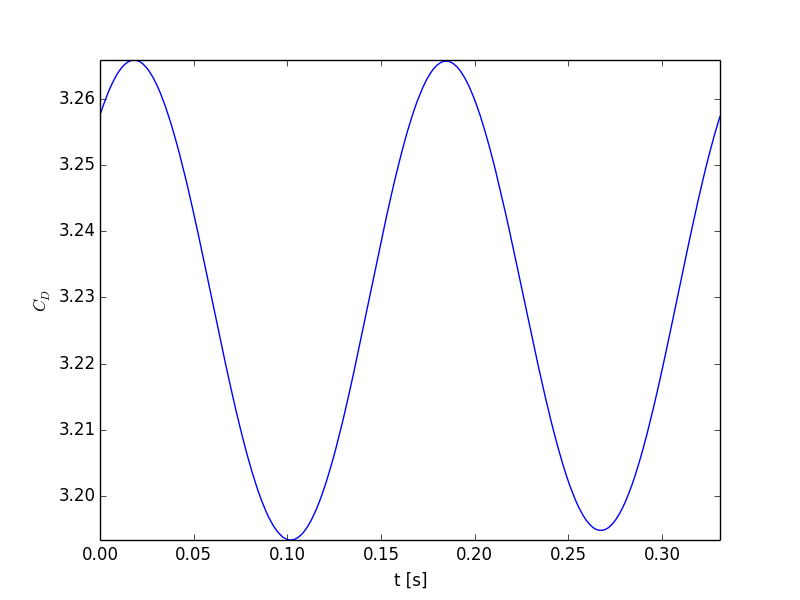
\includegraphics[scale=0.7]{2b_figure_1.png}
\end{figure}
\begin{figure}[h!]
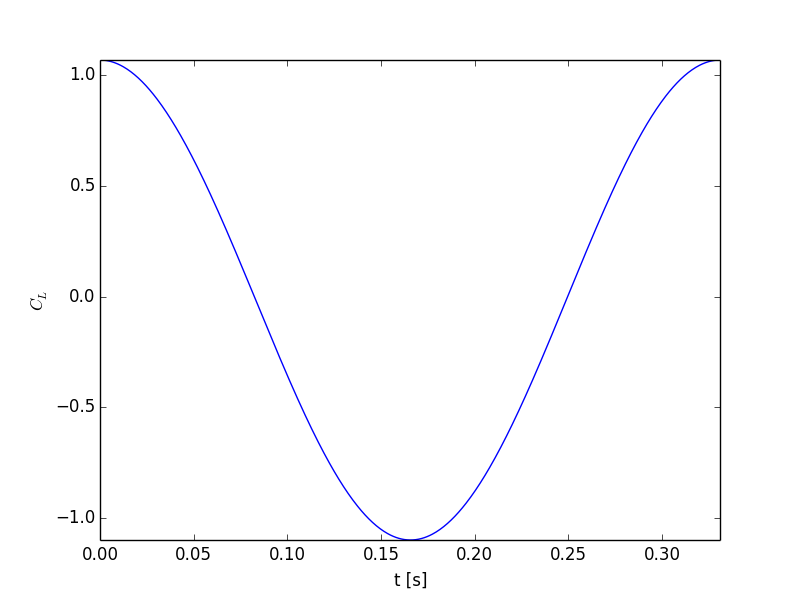
\includegraphics[scale=0.7]{2b_figure_2.png}
\end{figure}
\begin{figure}[h!]
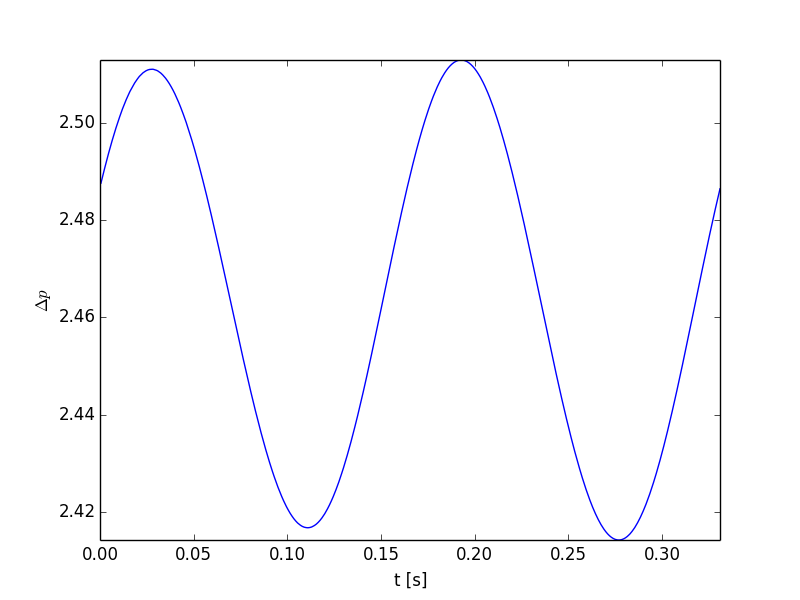
\includegraphics[scale=0.7]{2b_figure_3.png}
\end{figure}\\

\newpage
\section*{iii a)}
We start by calculating the pressure gradient from the momentum equation as described in Hint 1:\\
\\
$0 = \nu\frac{\partial^2\ol{u}}{\partial y^2} - \frac{1}{\rho}\frac{\partial\ol{p}}{\partial x} - \frac{\partial\ol{u'v'}}{\partial y}$\\
\\
$0 = \nu\int\limits_{-h}^h\frac{\partial^2\ol{u}}{\partial y^2}dy - \frac{1}{\rho}\frac{\partial\ol{p}}{\partial x}\int\limits_{-h}^hdy - \int\limits_{-h}^h\frac{\partial\ol{u'v'}}{\partial y}dy$\\
\\
$0 = \nu\frac{\partial\ol{u}}{\partial y}\Big|_{y=h} - \nu\frac{\partial\ol{u}}{\partial y}\Big|_{y=-h} - \frac{1}{\rho}\frac{\partial\ol{p}}{\partial x}\Big[y\Big]_{-h}^h - \left(\ol{u'v'}\Big|_{y=h} - \ol{u'v'}\Big|_{y=-h} \right)$\\
\\
\\
The term $\frac{\partial\ol{u}}{\partial y}$ will be negative at the upper wall and positive at the lower wall, so the first term equals $-{v^*}^2$ while the second equals ${v^*}^2$. The last two terms equal zero, so we end up with the equation:\\
\\
$0 = -2{v^*}^2 - \frac{2h}{\rho}\frac{\partial\ol{p}}{\partial x}$\\
\\
giving\\
\\
$\frac{1}{\rho}\frac{\partial\ol{p}}{\partial x} = -\frac{{v^*}^2}{h}$\\
\\
We insert this into the momentum equation and also replace the last term using the second and third identities given in the assignment:\\
\\
$0 = \nu\frac{\partial^2\ol{u}}{\partial y^2} + \frac{{v^*}^2}{h} - \frac{\partial}{\partial y}\left(-l^2\big|\frac{\partial\ol{u}}{\partial y}\big|\frac{\partial\ol{u}}{\partial y} \right)$\\
\\
We create a variational form by multiplying the equation by a test function v, and integrating over the domain:\\
\\
$0 = -\nu\int\limits_{\Omega}\nabla\ol{u}\cdot\nabla v dx + \frac{{v^*}^2}{h}\int\limits_{\Omega}v dx + l^2 \int\limits_{\Omega}\left(\frac{\partial}{\partial y}\left[\big|\frac{\partial\ol{u}}{\partial y}\big|\frac{\partial\ol{u}}{\partial y} \right]\right)v dx$\\
\\
Where the Lapace term has been integrated by parts as previously. The last term can also be integrated by parts:\\
\\
$\int\limits_{\Omega}\left(\frac{\partial}{\partial y}\left[\big|\frac{\partial\ol{u}}{\partial y}\big|\frac{\partial\ol{u}}{\partial y} \right]\right)v dx = - \int\limits_{\Omega}\big|\frac{\partial\ol{u}}{\partial y}\big|\frac{\partial\ol{u}}{\partial y} \frac{\partial v}{\partial y}dx + \big|\frac{\partial\ol{u}}{\partial y}\big|\frac{\partial\ol{u}}{\partial y}v\Big|_{-h}^{h}$\\
\\
where the last term is zero. The final variational form then becomes:\\
\\
$0 = -\nu\int\limits_{\Omega}\nabla\ol{u}\cdot\nabla v dx + \frac{{v^*}^2}{h}\int\limits_{\Omega}v dx - l^2\int\limits_{\Omega}\big|\frac{\partial\ol{u}}{\partial y}\big|\frac{\partial\ol{u}}{\partial y} \frac{\partial v}{\partial y}dx$\\
\\
\newpage
This can be solved using Newton iterations, and I have done so in the following code:\\
\\
\begin{lstlisting}[style=python]
from dolfin import *
from numpy import arctan, zeros
import matplotlib.pyplot as plt
set_log_active(False)

h = 1.
vs = 0.05
Re = 1000.
nu = vs/Re
k = 0.41
A = 26.

mesh = IntervalMesh(230, 0, h)
V = FunctionSpace(mesh, 'CG', 1)
ug = TrialFunction(V)
v = TestFunction(V)

bcs = DirichletBC(V, Constant(0), "std::abs(x[0]) < 1e-12")

x = mesh.coordinates()
xdiff = x[1]-x[0]
x[:,0] = h - (arctan(pi*(x[:,0])) / arctan(pi))
yplus = x*Re

l = Expression("k*x[0]*(1-exp(-x[0]*vs/(nu*A)))", k=k, vs=vs, 
			A=A, nu=nu)

Fg = nu*inner(grad(v), grad(ug))*dx - (vs**2/h)*v*dx


u_ = Function(V)
solve(lhs(Fg)==rhs(Fg), u_, bcs = [bcs])

F = nu*v.dx(0)*u_.dx(0)*dx - (vs**2/h)*v*dx + 
	l**2*abs(u_.dx(0))*u_.dx(0)*v.dx(0)*dx

solve(F==0, u_, bcs = [bcs])

uval = u_.compute_vertex_values()
uplus = uval/vs

plt.figure()
plt.plot(yplus,uplus)
plt.xlabel('$ y^+ $')
plt.ylabel('$ u^+ $')
plt.axis([0,5,0,5])

B = 5.5
u30 = interpolate(Expression("(1/k)*log(x[0]*Re) + B", k=k, 
		B=B, Re=Re),V)
u30vals = u30.compute_vertex_values()
plt.figure()
plt.plot(yplus,uplus, label = 'calculated solution')
plt.plot(yplus,u30vals, label = 'theoretical solution')
plt.legend(loc='center right')
plt.xlabel('$ y^+ $')
plt.ylabel('$ u^+ $')
plt.axis([30,1000, 0, 25])

B = 5
u30 = interpolate(Expression("(1/k)*log(x[0]*Re) + B", k=k, 
	B=B, Re=Re),V)
u30vals = u30.compute_vertex_values()
plt.figure()
plt.plot(yplus,uplus, label = 'calculated solution')
plt.plot(yplus,u30vals, label = 'theoretical solution')
plt.legend(loc='center right')
plt.xlabel('$ y^+ $')
plt.ylabel('$ u^+ $')
plt.axis([30,1000, 0, 25])

ll = interpolate(l,V)
lvals = ll.compute_vertex_values()
du = zeros(len(uval))

du = project(u_.dx(0),V)
print(du(1)*lvals[0])
plt.show()

\end{lstlisting}
This first solves the equation without the last term, and then uses the calculated solution as a guess for the Newton iterations for the complete equation.\\
\\
As we can see, we had to modify the mesh to 230 nodes to get the first internal node to give $y^+ < 1$. If we were to use a non-skewed mesh, we would need 1001 or more nodes to ensure that the first internal node is < 1.

\newpage
\section*{iii b)}
Running the program, we get the following plot for $y^+$ vs. $u^+$ for $y^+ < 5$:
\begin{figure}[h!]
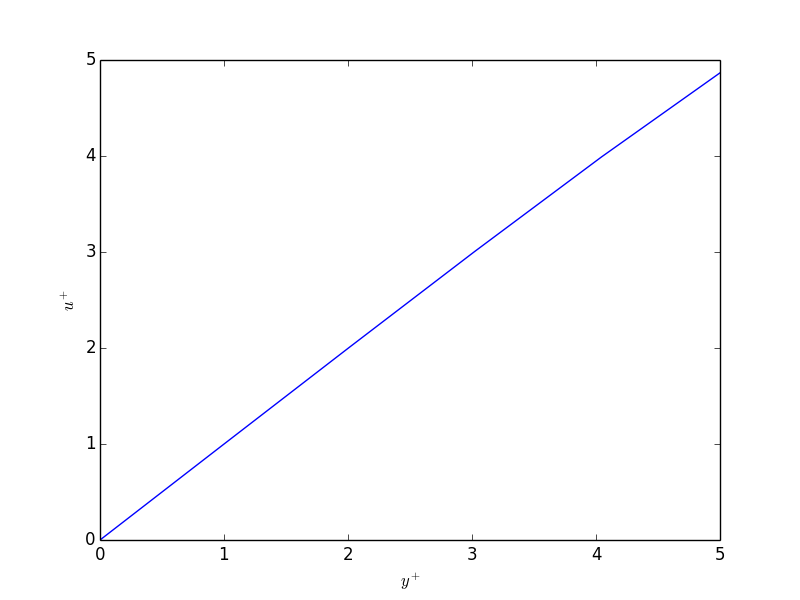
\includegraphics[scale=0.7]{3b_figure_1.png}
\end{figure}
\\
As we can see, this is fairly linear, so the computed solution approximates the theoretical result pretty well.\\
\\
\newpage
At $y^+$ > 30, the plot below shows the computed and theoretical solutions:
\begin{figure}[h!]
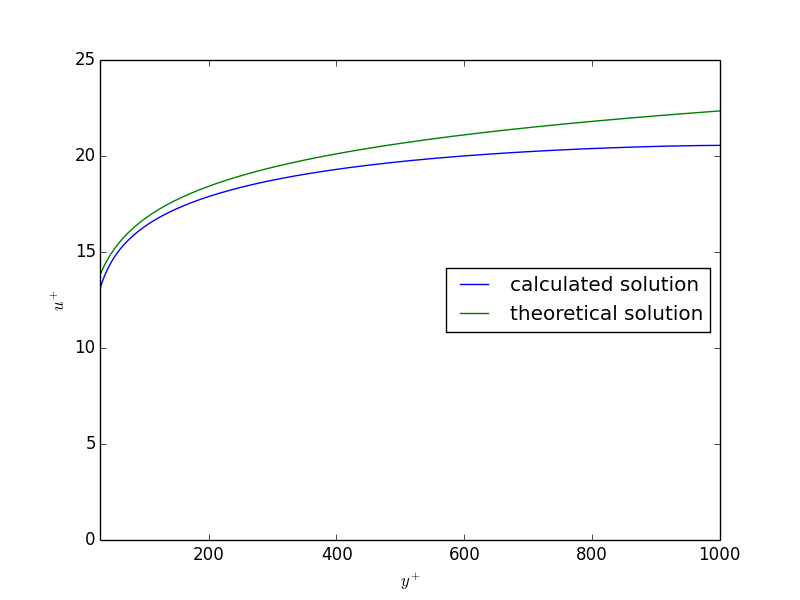
\includegraphics[scale=0.6]{3b_figure_2.png}
\end{figure}\\
Changing the constant B to 5, we get a closer match to the theoretical solution at the start of the plot:
\begin{figure}[h!]
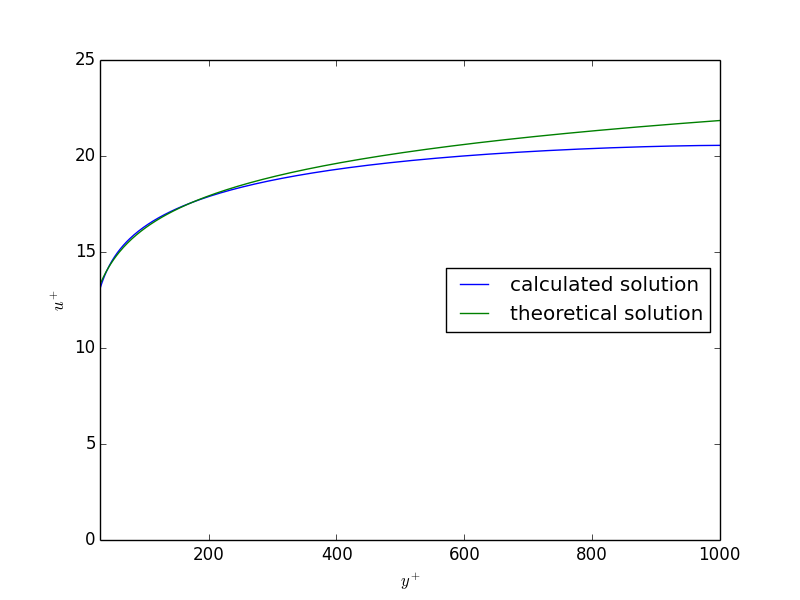
\includegraphics[scale=0.6]{3b_figure_3.png}
\end{figure}\\

\newpage
The value for the constant B for which I got the smalles error between the two solutions was around 4.409 (I cound not bother refining further!), giving the following plot:
\begin{figure}[h!]
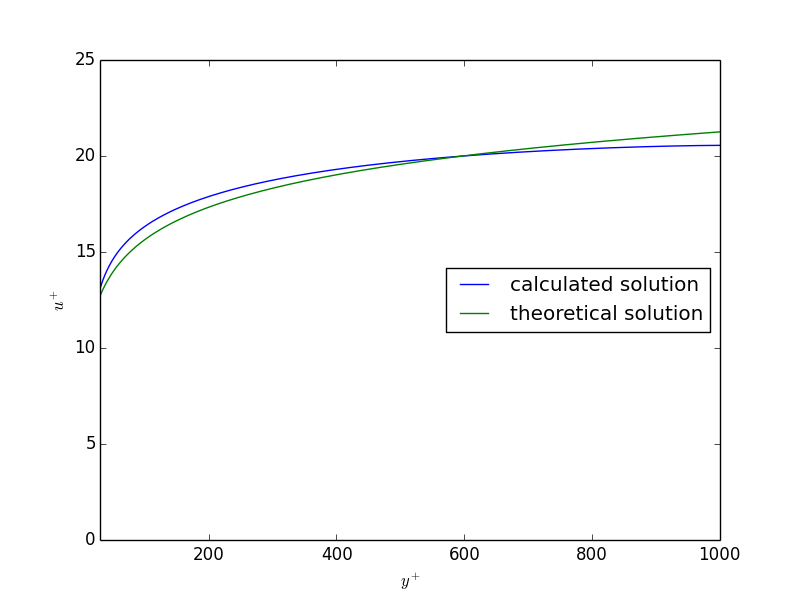
\includegraphics[scale=0.7]{3b_figure_4.png}
\end{figure}\\
Here the solutions lie close to each other at around $y^+ = 600$, but are further apart at the extremities.\\
\\
The program finally comutes the value for $\nu_T$, giving a value of 0.003. As this by definition shoud be zero at the center of the channel, we can conclude that the model is not entirely accurate.

\newpage
\section*{iv)}
We start with the derivation of the Reynolds Averaged Navier-Stokes equations. We first have the usual momentum and continuity equations (with index notation):\\
\\
(1)$\tab \rho\left[\pdi{u_i}{t} + u_j\pdi{u_i}{x_j}\right] = -\pdi{p}{x_i} + \pdi{\tau_{ij}}{x_j}$\\
\\
(2)$\tab\pdi{u_j}{x_j} = 0$\\
\\
where for clarity\\ 
\\
$\tau_{ij} = \mu\left[\pdi{u_i}{x_j} + \pdi{u_j}{x_i} \right]$\\
\\
We want to decompose the flow into two parts, the mean flow and the fluctuation. We define:\\
\\
$u_i = \ol{u_i} + u_i'$\\
\\
where $\ol{u_i}$ is the mean flow and $u_i'$ is the fluctuation. From the book we have that averaging and differentiation commutes:\\
\\
$\pdi{u_i}{t} = \pdi{\ol{u_i}}{t}$\\
\\
Also, the mean of the fluctuation is zero:\\
\\
$\ol{u_i} = 0$\\
\\
And finally we have the following identities:\\
\\
$\ol{\ol{u_i}} = \ol{u_i},\tab\ol{u_i\ol{u_j}} = \ol{u_i}\ol{u_j},\tab\ol{u_i'\ol{u_i}} = 0,\tab\ol{u_i + u_j} = \ol{u_i} + \ol{u_j},\tab\ol{u_i u_j} = \ol{u_i}\ol{u_j} + \ol{u_i' u_j'}$\\
\\
Now by replacing the instantaneous values in (1) by the decompositions, we get:\\
\\
(2)$\tab \rho\left[\pdi{(\ol{u_i} + u_i')}{t} + (\ol{u_j} + u_j')\pdi{(\ol{u_i} + u_i')}{x_j}\right] = -\pdi{(\ol{p} + p')}{x_i} + \pdi{(\ol{\tau_{ij}} + \tau_{ij}')}{x_j}$\\
\\
We average the equation:\\
\\
$\ol{\rho\left[\pdi{(\ol{u_i} + u_i')}{t} + (\ol{u_j} + u_j')\pdi{(\ol{u_i} + u_i')}{x_j}\right] = -\pdi{(\ol{p} + p')}{x_i} + \pdi{(\ol{\tau_{ij}} + \tau_{ij}')}{x_j}}$\\
\\
And by using the identites and commuting rules stated above, this reduces to (convection term expanded for clarity):\\
\\
$\rho\left[\pdi{\ol{u_i}}{t} + \ol{\ol{u_j}\pdi{\ol{u_i}}{x_j}} + \ol{\ol{u_j}\pdi{u_i'}{x_j}} + \ol{u_i'\pdi{\ol{u_i}}{x_j}} + \ol{u_i'\pdi{u_i'}{x_j}}\right] = -\pdi{\ol{p}}{x_i}+ \pdi{\ol{\tau_{ij}}}{x_j}$\\
\\
Here, the two middle terms in the left bracket equal zero. By rearanging the terms, we get the  following equation:\\
\\
(3)$\tab\rho\left[\pdi{\ol{u_i}}{t} + \ol{u_j}\pdi{\ol{u_i}}{x_j}\right] = -\pdi{\ol{p}}{x_i}+ \pdi{\ol{\tau_{ij}}}{x_j} - \rho\ol{u_j'\pdi{u_i'}{x_j}}$\\
\\
We then substitute the decompostition into the continuity equation:\\
\\
$\pdi{(\ol{u_j} + u_j')}{x_j} = 0$\\
\\
Giving the averaged continuity eqaution:\\
\\
$\pdi{\ol{u_j}}{x_j} = 0$\\
\\
Subtracting the second of these equations from the first, we can get the identity:\\
\\
$\pdi{u_j'}{x_j} = 0$\\
\\
If we multiply this by $u_i'$ and average, we get:\\
\\
$\ol{u_i'\pdi{u_j'}{x_j}} = 0$\\
\\
This can be used in the following way:\\
\\
$\ol{u_j'\pdi{u_i'}{x_j}} + 0 = \ol{u_j'\pdi{u_i'}{x_j}} + \ol{u_i'\pdi{u_j'}{x_j}} = \pdi{}{x_j}\ol{u_i' u_j'}$\\
\\
Using this to replace the last term in (3) and combining the two last terms, we get the equivalent version of equation 6-13 in White:\\
\\
$\rho\left[\pdi{\ol{u_i}}{t} + \ol{u_j}\pdi{\ol{u_i}}{x_j}\right] = -\pdi{\ol{p}}{x_i}+ \pdi{}{x_j}\left[\ol{\tau_{ij}} - \rho\ol{u_i' u_j'}\right]$\\
\\
\\
\\
\\
Next we want to derive the Reyolds Stress Equation. We start by simply subtracting equation (3) from equation (2):\\
\\
$\rho\left[\pdi{u_i'}{t} + \ol{u_j}\pdi{u_i'}{x_j} + u_j'\pdi{\ol{u_i}}{x_j} + u_j'\pdi{u_i'}{x_j}\right] = -\pdi{p'}{x_i} + \pdi{\tau_{ij}'}{x_j} + \rho\ol{u_j'\pdi{u_i'}{x_j}}$\\
\\
Which we rewrite as:\\
\\
$\rho\left[\pdi{u_i'}{t} + \ol{u_j}\pdi{u_i'}{x_j}\right] = -\pdi{p'}{x_i} + \pdi{\tau_{ij}'}{x_j} - \rho u_j'\pdi{\ol{u_i}}{x_j} - \rho\left[u_j'\pdi{u_i'}{x_j} - \ol{u_j'\pdi{u_i'}{x_j}}\right]$\\
\\
Next we mulitply this by $u_k'$ and average:\\
\\
(4)$\tab\rho\left[\ol{u_k'\pdi{u_i'}{t}} + \ol{u_j}\ol{u_k'\pdi{u_i'}{x_j}}\right] = -\ol{u_k'\pdi{p'}{x_i}} + \ol{u_k'\pdi{\tau_{ij}'}{x_j}} - \rho\left[\ol{u_k' u_j'}\pdi{\ol{u_i}}{x_j}\right] - \rho\left[\ol{u_k' u_j'\pdi{u_i'}{x_j}}\right]$\\
\\
The indices i and k can be interchanged, so we can rearrange to get another equation:\\
\\
(5)$\tab\rho\left[\ol{u_i'\pdi{u_k'}{t}} + \ol{u_j}\ol{u_i'\pdi{u_k'}{x_j}}\right] = -\ol{u_i'\pdi{p'}{x_k}} + \ol{u_i'\pdi{\tau_{kj}'}{x_j}} - \rho\left[\ol{u_i' u_j'}\pdi{\ol{u_k}}{x_j}\right] - \rho\left[\ol{u_i' u_j'\pdi{u_k'}{x_j}}\right]$\\
\\
Adding (4) and (5) together, we get:\\
\\
(6)$\tab\pdi{\ol{u_i' u_k'}}{t} + \ol{u_j}\pdi{\ol{u_i' u_k'}}{x_j} = -\frac{1}{\rho}\left[\ol{u_i'\pdi{p'}{x_k}} + \ol{u_k'\pdi{p'}{x_i}}\right] - \left[\ol{u_i' u_j'\pdi{u_k'}{x_j}}\ + \ol{u_k' u_j'\pdi{u_i'}{x_j}}\right] + \frac{1}{\rho}\left[\ol{u_i'\pdi{\tau_{kj}'}{x_j}} + \ol{u_k'\pdi{\tau_{ij}'}{x_j}}\right]\\\\\tab\tab\tab\tab\tab\tab - \left[\ol{u_i' u_j'}\pdi{\ol{u_k}}{x_j} + \ol{u_k' u_j'}\pdi{\ol{u_i}}{x_j}\right]$\\
\\
We rewrite the first term on the right hand side of (6):\\
\\
$\left[\ol{u_i'\pdi{p'}{x_k}} + \ol{u_k'\pdi{p'}{x_i}}\right] = - \ol{p'\left[\pdi{u_i'}{x_k} + \pdi{u_k'}{x_i}\right]} + \pdi{}{x_j}\left[\ol{p' u_i'}\delta_{kj} + \ol{p' u_k'}\delta_{ij}\right]$\\
\\
Where $\delta_{ij}$ is the Kronecker delta. We also rewrite the third term on the right hand side of (6):\\
\\
$\left[\ol{u_i'\pdi{\tau_{kj}'}{x_j}} + \ol{u_k'\pdi{\tau_{ij}'}{x_j}}\right] = - \left[\ol{\tau_{ij}\pdi{u_k'}{x_j}} + \ol{\tau_{kj}\pdi{u_i'}{x_j}}\right] + \pdi{}{x_j}\left[\ol{u_i'\tau_{kj}}  + \ol{u_k'\tau_{ij}}\right]$\\
\\
And use the fact that:\\
\\
$\tau_{ij}' = 2\mu s_{ij}'$, where $s_{ij}' = \frac{1}{2}\left[\pdi{u_i'}{x_j} + \pdi{u_j'}{x_i}\right]$\\
\\
to get:\\
\\
$\frac{1}{\rho}\left[\ol{\tau_{ij}\pdi{u_k'}{x_j}} + \ol{\tau_{kj}\pdi{u_i'}{x_j}}\right] = 2\nu\left[\ol{s_{ij}'\pdi{u_k'}{x_j}} + \ol{s_{kj}'\pdi{u_i'}{x_j}}\right]$\\
\\
$\pdi{}{x_j}\left[\frac{1}{\rho}\ol{u_i'\tau_{kj}}  + \ol{u_k'\tau_{ij}}\right] = \pdi{}{x_j}\left[2\nu\left(\ol{u_i's_{kj}'}  + \ol{u_k's_{ij}'}\right)\right]$\\
\\
Finally we rewrite the second term on the right-hand side of (6):\\
\\
$\left[\ol{u_i' u_j'\pdi{u_k'}{x_j}}\ + \ol{u_k' u_j'\pdi{u_i'}{x_j}}\right] = \pdi{}{x_j}\ol{u_i' u_k' u_j'}$\\
\\
Inserting all the rewritten terms into (6), we get the Reynolds Stress Equation:\\
\\
(7)$\tab\pdi{\ol{u_i' u_k'}}{t} + \ol{u_j}\pdi{\ol{u_i' u_k'}}{x_j} = \ol{p'\left[\pdi{u_i'}{x_k} + \pdi{u_k'}{x_i}\right]} + \pdi{}{x_j}\left\{-\frac{1}{\rho}\left[\ol{p' u_i'}\delta_{kj} + \ol{p' u_k'}\delta_{ij}\right]- \ol{u_i' u_k' u_j'} + 2\nu\left[\ol{u_i's_{kj}'}  + \ol{u_k's_{ij}'}\right]\right\}\\
\tab\tab\tab \tab\tab- \left[\ol{u_i' u_j'}\pdi{\ol{u_k}}{x_j} + \ol{u_k' u_j'}\pdi{\ol{u_i}}{x_j}\right] - 2\nu\left[\ol{s_{ij}'\pdi{u_k'}{x_j}} + \ol{s_{kj}'\pdi{u_i'}{x_j}}\right]$\\
\\
Comparing this to 6-18 in White, we see that these are equal with the interchanging of incices j and k, and some further rewriting of the term $s_{ij}.'$\\
\\
\\
\\
\\
Finally we look to find the Turbulence Kinetic-Energy Equation. Looking at the derivation in the online book, I was not able to follow the steps in my mind all the way through, but it is anyhow reproduced bellow. The book starts by contracting the free indices in (7), giving:\\
\\
(8)$\tab\pdi{\ol{u_i' u_i'}}{t} + \ol{u_j}\pdi{\ol{u_i' u_i'}}{x_j} = \pdi{}{x_j}\left\{-\frac{2}{\rho}\ol{p' u_i'}\delta_{ij} - \ol{u_i' u_i' u_j'} + 4\nu\ol{u_i's_{ij}'}\right\} - 2\ol{u_i' u_j'}\pdi{\ol{u_i}}{x_j} - 4\nu\ol{s_{ij}'\pdi{u_i'}{x_j}}$\\
\\
Where we have used that $\pdi{u_i}{x_i} = 0$ to get rid of the first righ-hand term in (7). Next the last term in (8) is rewritten using:\\
\\
$\ol{s_{ij}'\pdi{u_i'}{x_j}} = \ol{s_{ij}'s_{ij}'}$\\
\\
using symmetric and anti-symmetric tensor relations as arguments. The term $k = \frac{1}{2}\ol{u_i'u_i'}$ is introduced, as in White. (8) is then rewritten as:\\
\\
(9)$\tab\left[\pdi{}{t} + \ol{u_j}\pdi{}{x_j}\right]k = \pdi{}{x_j}\left\{-\frac{1}{\rho}\ol{p' u_i'}\delta_{ij} - \frac{1}{2}\ol{u_i' u_i' u_j'} + 2\nu\ol{u_i's_{ij}'}\right\} - \ol{u_i' u_j'}\pdi{\ol{u_i}}{x_j} - 2\nu\ol{s_{ij}'s_{ij}'}$\\
\\
This is the derived form of the Turbulence Kinetic-Energy Equation as given in the online book. Comparing this to 6-17 in White we can see the equivalent terms, once again with a different index notation and expanded $s_{ij}'$ terms.

 \end{document}
